\begin{figure}[htb]
\begin{center}
  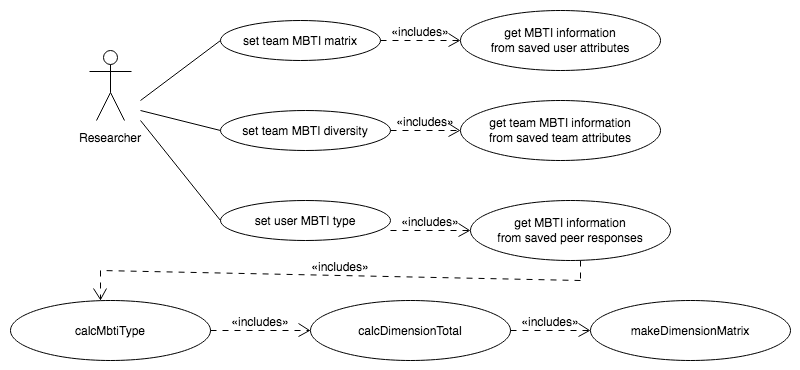
\includegraphics[width=\textwidth,keepaspectratio=true]{MBTIscope}
\end{center}
\caption{Services related to the MBTI personality types of users and teams\label{fig:mbti_functionalRequirements}}
\end{figure}

Figure \ref{fig:mbti_functionalRequirements} shows the lower level services required by the services related to the MBTI personality types of users. The services are the following:

\begin{description}

\item[setMbtiType] The service takes the userID as parameter and returns the MBTI type of the user. The result is a four character acronym identifying MBTI type of the user. The calculated value in the dimension matrix returned by the \texttt{makeDimensionMatrix} function for the user is used to assign the dimension category to the user. If the value is negative the \textit{left letter} describing the dimension is assigned and if it is positive, then the \textit{letter on the right} is assigned. If the dimension is empty or zero, the dimension is taken as neutral. If empty it is indicated with `-' while zero is indicated with `*'.  The identified MBTI personality type of the user should be persisted in the user profile of the user using the \texttt{setMBTIAttributes} service described in Section~\ref{userAttributes}.

\item[setTeamMBTIMatrix] The service takes the teamID as parameter and create a mbti object for the team. The object consist of four columns and three rows of integer values. The columns represent the four MBTI personality type dimensions. The rows represent counts for the dimension characters  i.e. the \textit{left}, \textit{neutral} and \textit{right} counts for each of the dimensions. The values are determined using the \texttt{getMBTIAttributes} service described in Section~\ref{userAttributes} for each each member in the team. The number of users in the team who has the dimension character is counted for each of the three dimension charcters of the dimension. For example in the \textbf{IE} dimension, the left count is the number of members of `I' type, the neutral is the number of members of `*' or `-' type and the right is the number of members of `E' type. The object is persisted as a team attribute using the \texttt{setTeamMBTIMatrix} described in Section~\ref{teamAttributes}.

\item[setMBTIdiversity] The service takes the teamID as parameter and returns a real value representing the personality diversity of the team. The matrix created by the  as described in Section~\ref{mbtiDiversity}. The resulting value is persisted as a team attribute using the \texttt{setTeamMBTIDiversity} described in Section~\ref{teamAttributes}.
\end{description}  


The following are helper functions used by the above services
\begin{description}

\item[calcMbtiType] This function takes the userID as parameter and returns the MBTI type of the user. The result is a four character acronym identifying MBTI type of the user. The calculated value in the dimension matrix of the user is used to assign the dimension category to the user. If the value is negative the left letter describing the dimension is assigned and if it is positive, then the letter on the right is assigned. If the dimension is empty or zero, the dimension is taken as neutral. If empty it is indicated with `-' while zero is indicated with `*'.  The identified MBTI personality type of the user should be persisted in the user profile of the user using the \texttt{setMBTIAttributes} service described in Section~\ref{userAttributes}.

\item[calcDimensionTotal] The function takes a MBTI dimension and a userID as parameters and determine the total weight for the dimension for the user assigned by respondents who have rated the user on this dimension. The responses to the question for the specific dimension is used to gather a list of ratings for the particular user. If the list is empty an exception is raised, otherwise each of the MBTI ratings are converted to numbers ranging from -3 to +3 with the first letter of the dimension being negatives and the last ones being positive; see the (Table~\ref{ab:mbti_ratings})  The return value is an integer calculated as the total of the assigned values.

\item[makeDimensionMatrix] The function takes the userID as parameter and create a mbti object for the user. The object consist of four integer values; one for each of the four MBTI personality dimension. The values are determined using the \texttt{calcDimensionTotal} function for each of the dimensions. If the function raises an exception, the dimension value remains empty, otherwise the returned integer is stored for the dimension. The function returns a vector of four integer values.


\end{description}  


\begin{table}[h]
\centering
\caption{Values assigned to MBTI personality type ratings \label{tab:mbti_ratings}}
\begin{tabular}{cc|cc|cc|cc}

\hline
\noalign{\smallskip}
\multicolumn{2}{c}{\textbf{IE}}  & \multicolumn{2}{c}{\textbf{SN}} & \multicolumn{2}{c}{\textbf{TF}} & \multicolumn{2}{c}{\textbf{JP}} \\
~Code~ & ~Value~ & ~Code~ & ~Value~ & ~Code~ & ~Value~ & ~Code~ & ~Value~\\
\noalign{\smallskip}
\hline
E++ & -3  & S++ & -3 & T++ & -3 & J++ & -3\\
E+ & -2 & S+ & -2 & T+ & -2 & J+ & -2  \\
E & -1 & S & -1 & T & -1 & J & -1  \\
I & 1 & N & 1 & F & 1 & P & 1 \\
I+ & 2  & N+ & 2 & F+ & 2 & P+ & 2 \\
I++ & 3 & N++  & 3 & F++  & 3 & P++  & 3 \\
\hline
\end{tabular}
\end{table}






